\documentclass[a4j]{ujarticle}
\usepackage[dvipdfmx]{graphicx}
\usepackage{url}
\usepackage{bbding}
\usepackage{lscape}


\title{進捗報告資料}
\author{安達智哉\\to-adachi@ist.osaka-u.ac.jp}
\date{平成30年12月13日}

\begin{document}
\maketitle

\section{アタッチの回数を削減することによりコントロールプレーンの負荷を減らすモデル(案)}
現在、負荷分散に基づくモバイルコアネットワークの性能向上方法について研究をしている途中であるが、前回のミーティングで村田先生がおっしゃった "アイディア勝負" というアドバイスを受け、一度、自分の研究を最初から見直してみた。その結果、負荷分散以外の方法でも、私の研究の目的(より多くのIoT端末を収容できるモバイルネットワークの考案)を達成できるのではないかと考えた。



\subsection{概要}
多数のM2M/IoT端末を収容することにより、コントロールプレーンの輻輳の問題が発生すると考えられている。その理由はM2M/IoT通信の通信特性にあり、M2M/IoT端末のように周期性や間欠性を持つ端末を収容する場合、データの送信ごとにアタッチ処理を行う必要があるため、コントロールプレーンに負荷が発生するからである。

そこで、本来ならデタッチ処理が行われるタイミングであっても、あえてデタッチ処理を行わないようにすることで、この問題を回避できるのではないかと考えた。つまり、M2M/IoT端末がデータの送信を終え、電源をOFFにした後も、セッションはそのまま維持しつつける。そして、M2M/IoT端末が再びONになりデータを送信する際には、以前と同じベアラを用いてデータを送信する。この方法によって、最初に一度アタッチ処理を行えば、その後のデータ送信においては、アタッチ処理は発生しないで済むため、コントロールプレーンの負荷軽減が期待できる。

\subsection{説明}
図\ref{detach-ON}は、M2M/IoT端末が最初にネットワークに接続した際の様子を示す。通常通り、アタッチの処理を行い、ベアラを確立する。図\ref{detach-OFF}は、M2M/IoT端末がネットワークから切断された際の様子を示す。通常と異なり、デタッチ処理が行われないため、ベアラはそのまま維持される。図\ref{detach-reON}はM2M/IoT端末が再びネットワークに接続した時の様子を示す。この場合、以前使用したベアラが残っているため、M2M/IoT端末はアタッチ処理をスキップしてデータの送受信を開始できる。

\begin{figure}[htbp]
	\centering
	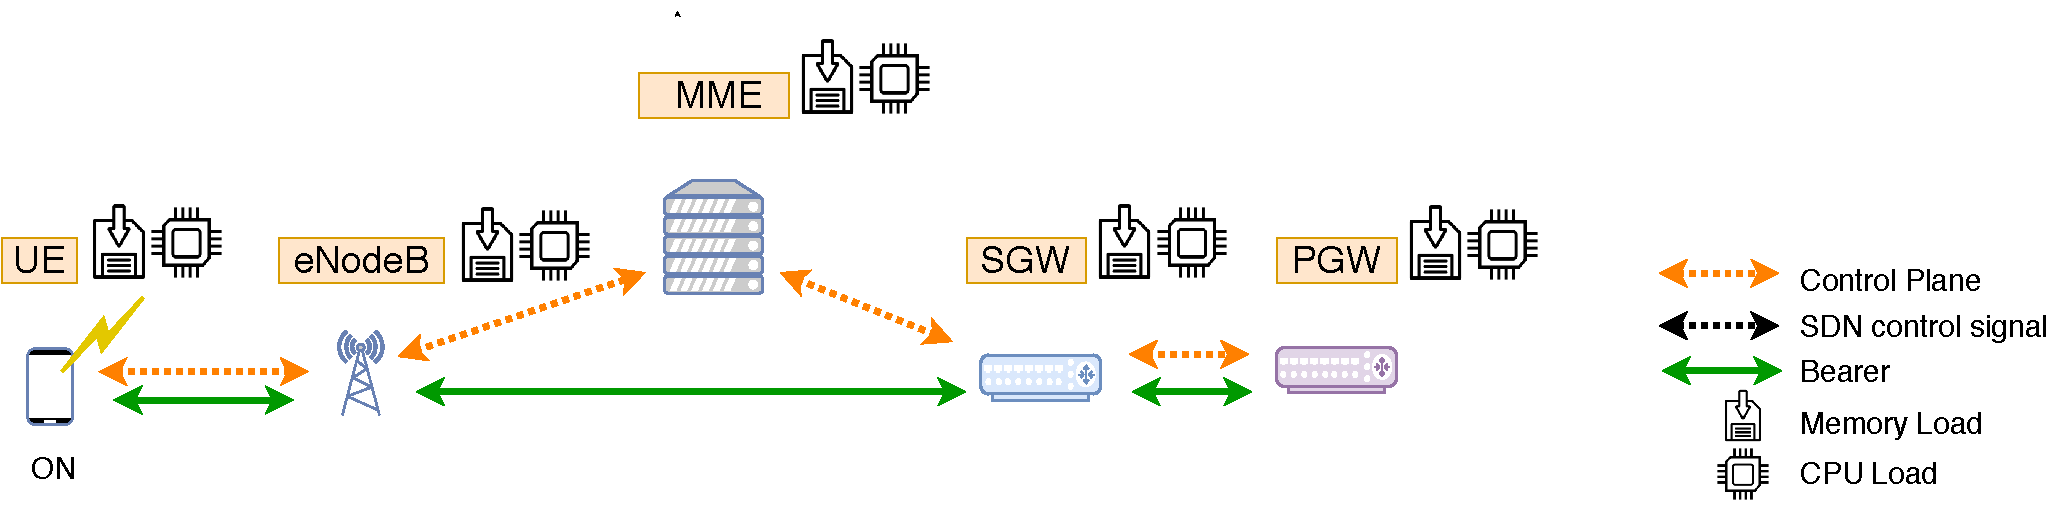
\includegraphics[width=0.7\hsize]{detach-ON.pdf}
  \caption{端末が最初にネットワークに接続した時と処理}
	\label{detach-ON}
\end{figure}

\begin{figure}[htbp]
	\centering
	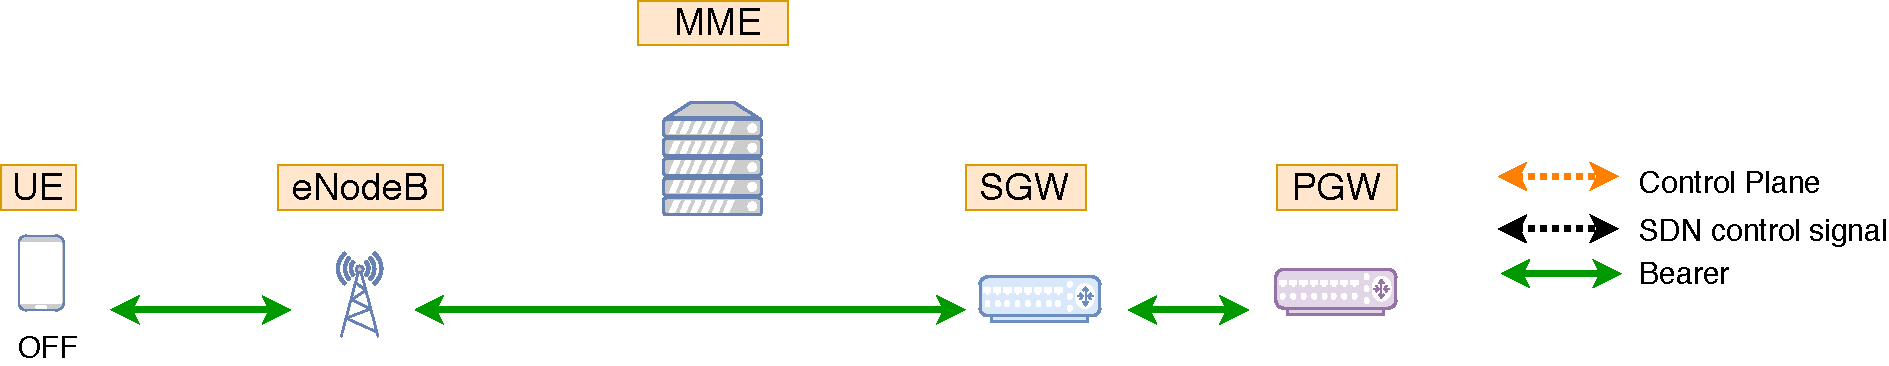
\includegraphics[width=0.7\hsize]{detach-OFF.pdf}
  \caption{端末がネットワークから切り離された時の処理}
	\label{detach-OFF}
\end{figure}

\begin{figure}[htbp]
	\centering
	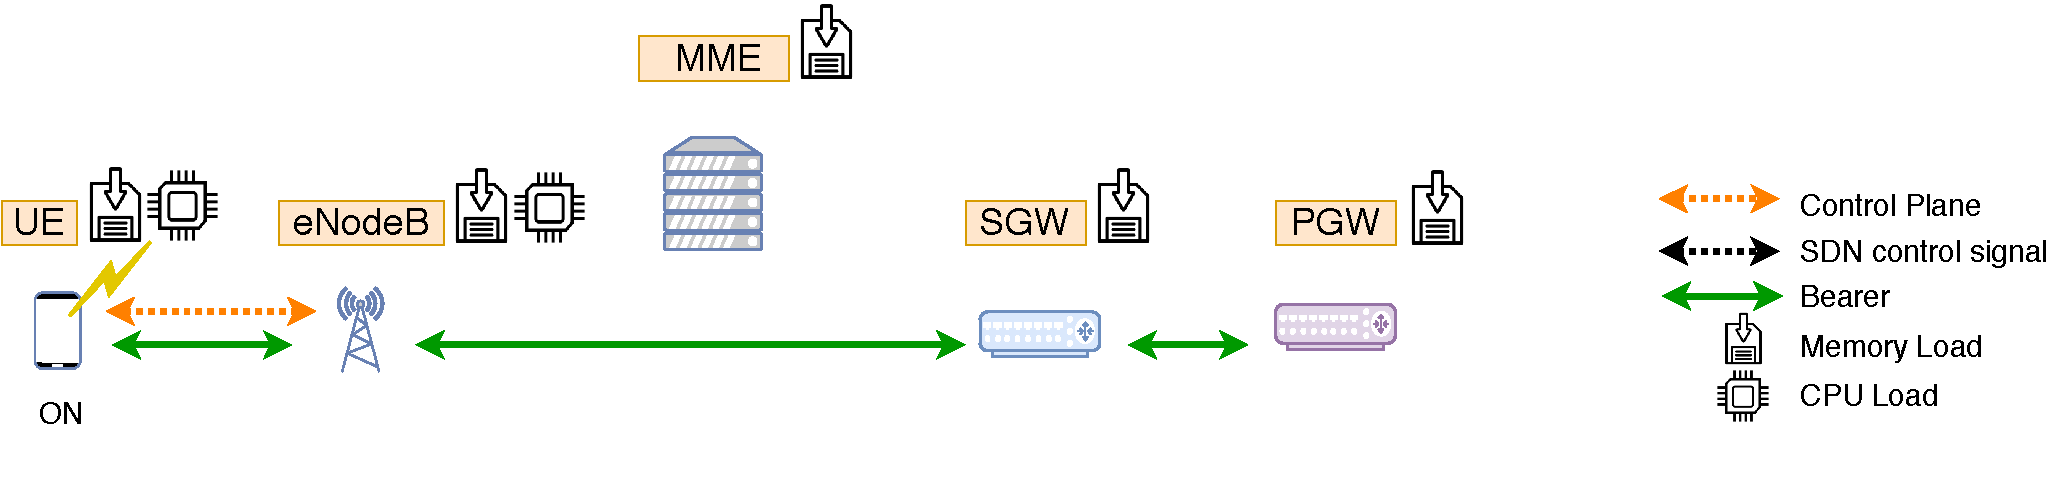
\includegraphics[width=0.7\hsize]{detach-reON.pdf}
  \caption{端末が2回目以降にネットワークに接続した時の処理}
	\label{detach-reON}
\end{figure}

\clearpage
eNodeB、MME、SGWおよびPGWは、ネットワークに接続されていないM2M/IoT端末のセッション情報を保持する必要があるため、リソース(主にメモリ)が圧迫されることが予想される。また、場合によっては、端末に割り当てるIPアドレスの枯渇などが発生する可能性もある。そのような、事態が発生した場合は、セッション情報がもっとも古い端末(最後にデータを送受信したタイミングが最も古い端末)から優先的にデタッチ処理を行い、リソースを解放する。

\subsection{利点}
上述の方法で、アタッチ処理を行う回数を減らすことで、M2M/IoT端末によるコントロールプレーンの負荷の増大に対して、根本的でかつ効果的な対策ができるのではないかと思う。負荷の原因そのものを削減できる点は、負荷分散などの他の方式と比較した際に強みであると思う。


%
% \section{今後の予定}
%
% \begin{itemize}
%   \item I/O待ち時間の調査を行う。具体的には先行研究論文や富士通株式会社などが公開しているサーバパフォーマンスに関するホワイトペーパーなどを参考にする。
% 	% \item PCRFの配置および課金処理の実現方法についての調査。
% \end{itemize}

\section*{\addcontentsline{toc}{section}{参考文献}}
{\scriptsize
\bibliographystyle{IEEEtran}
\bibliography{/Users/t-adachi/Documents/study/Bibliography/bib/hpt_core_network/myBib/LABbiblio,/Users/t-adachi/Documents/study/Bibliography/bib/hpt_core_network/Study_Group_Bibtex/bib/hptCoreNetwork_Study}
}
\end{document}
